\chapter{\label{chap:chap4} Metodologia e cronograma de desenvolvimento}
Para construção do projeto utilizaremos Python\cite{python}, em sua versão 3.x, como linguagem de programação.
Mais precisamente, utilizaremos a interface de baixo nível de rede da biblioteca padrão da linguagem \cite{socketPython}.
Algumas ferramentas para auxiliar o desenvolvimento serão utilizadas, como Visual Studio Code\cite{vscode} para edição de código e GitHub\cite{github} para o versionamento.

O cronograma deste trabalho foi baseado em iterações semanais como pode ser observado abaixo.
\begin{figure}[htb!]
    \centering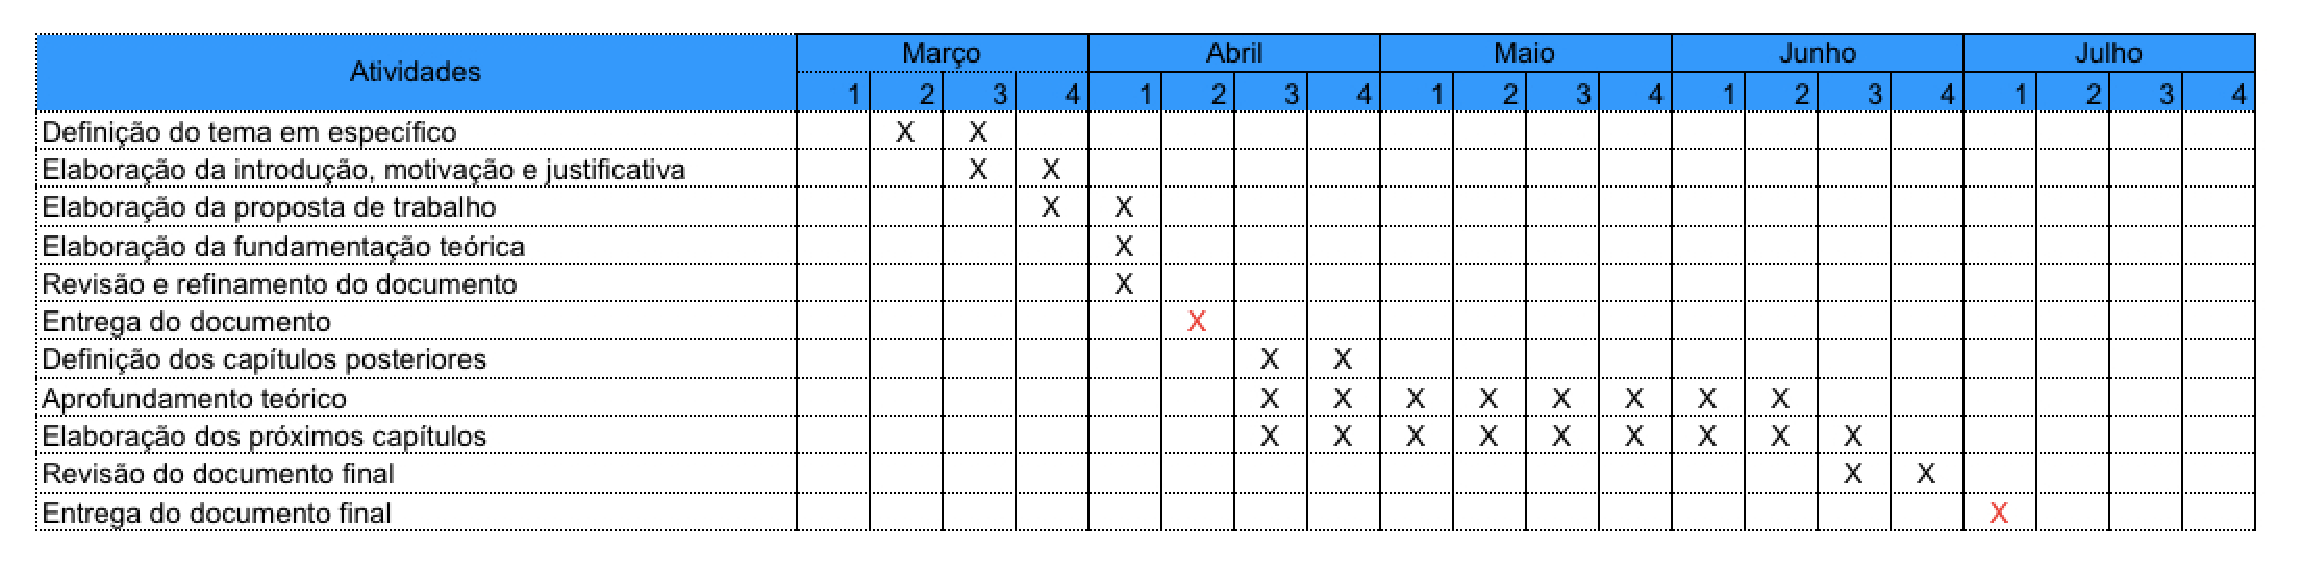
\includegraphics[width=1\textwidth]{fig3.pdf}
    \caption%[This figure has a shorter caption now]%
    {\label{fig:fig3} Cronograma de atividades.}
\end{figure}



